 \documentclass{article}
\usepackage{multiGWAS-preamble}

\begin{document}

\title{MultiGWAS: An integrative tool for Genome Wide Association Studies (GWAS) in tetraploid organisms}

\author[1]{L. Garreta}
\author[1]{I. Cer\'{o}n-Souza}
\author[2]{M.R. Palacio}
\author[1]{P.H. Reyes-Herrera}

\affil[1]{Corporaci\'{o}n Colombiana de Investigaci\'{o}n Agropecuaria (AGROSAVIA), CI Tibaitat\'{a},  Kil\'{o}metro 14, V\'{i}a a Mosquera, 250047, Colombia}

\affil[2]{Corporaci\'{o}n Colombiana de Investigaci\'{o}n Agropecuaria (AGROSAVIA), CI El Mira, Kil\'{o}metro 38, V\'{i}a Tumaco Pasto, Colombia}


\maketitle

%%226/250
%Aquí hice unos cambios pequeños para ampliar el espectro del estudio a cualquier planta tetraploide ya que esta revista está enfocada en herramientas para estudios evolutivos de cualquier organismo. Att. Ivaniahttps://www.overleaf.com/project/5e8b8de6ae23ed0001a9a14f

\begin{abstract}
\textbf{Summary:} The Genome-Wide Association Studies (GWAS) are essential to determine the association between genetic variants across individuals. One way to support the results is by using different tools to validate the reproducibility of the associations. Currently, software for GWAS in diploids is well-established but for polyploids species is scarce. Each GWAS software has its characteristics, which can cost time and effort to use them successfully. Here, we present MultiGWAS, a tool to do GWAS analysis in tetraploid organisms by executing in parallel and integrating the results from four existing GWAS software: two available for polyploids (GWASpoly and SHEsis) and two frequently used for diploids (PLINK and TASSEL). The tool deals with all the elements of the GWAS process in the four software, including (1) the input and conversion between genotypic data file formats (2) the use of different control quality filters for the genomic data, (3) the execution of two GWAS models, the full model with control for population structure and individual relatedness and the Naive model without any control. (4) The integration and reporting of results. The summary report generated by MultiGWAS provides the user with tables and plots describing intuitively the significant association found by both each one and across four software, which helps users to check for false-positive or false-negative results.\\
MultiGWAS generates five summary results integrating the four tools. (1) Score tables with detailed information on the associations for each tool. (2) Venn diagrams of shared SNPs among the four tools. (3) Heatmaps of significative SNP profiles among the four tools. (4) Manhattan and QQ plots for the association found by each tool. And (5) Chord diagrams for the chromosomes vs. SNP by each tool.%PAULA: no se si explicamos un poco mejor el output acA?\\
\\
\textbf{Contact:} phreyes@agrosavia.co\\
\textbf{Keywords: GWAS, tetraploids, SNPs, polyploids, software}
\end{abstract}

\maketitle 

% Preview source code from paragraph 2 to 10


\section{Introduction}

The Genome-wide association studies (GWAS) are used to identify which variants through the whole genome of a large number of individuals are associated with a specific trait (\cite{cantor2010prioritizing,begum2012comprehensive}). This methodology started with humans and several model plants, such as rice, maize, and \emph{Arabidopsis} (\cite{lauc2010genomics,tian2011genome,cao2011whole,korte2013advantages,han2013sequencing}). Because of the advances in the next-gen sequencing technology and the decline of the sequencing cost in recent years, there is an increase in the availability of genome sequences of different organisms at a faster rate (\cite{ekblom2011applications,ellegren2014genome}). Thus, the GWAS is becoming the standard tool to understand the genetic bases of either ecological or economic phenotypic variation for both model and non-model organisms. This increment includes complex species such as polyploids (Fig. \ref{GWASpolyploids}) (\cite{ekblom2011applications,santure2018wild}).

% Figure timelines articles
\begin{figure}[H]
\begin{centering}
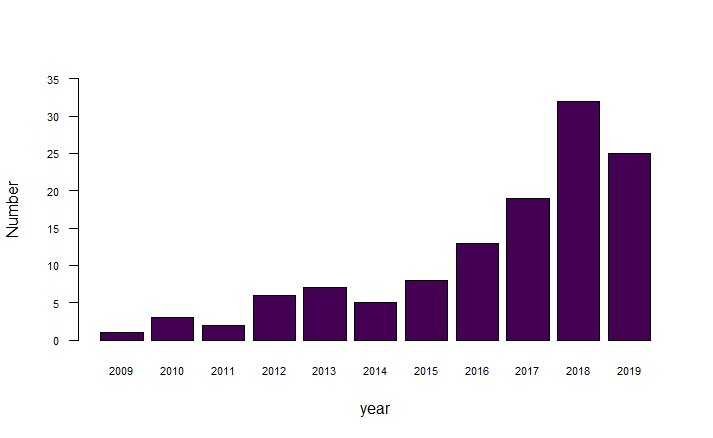
\includegraphics[width=10cm]{images/GWASpolyploids_Pubmed.png} 
\par\end{centering}
\centering{}\caption{Figure 1. The number of peer-reviewed papers that contains the keywords "GWAS" and "polyploid" in the PubMed database between 2009 and 2019.\label{GWASpolyploids}}
\end{figure}

The GWAS for polyploid species has fourth related challenges. First, as all GWAS, we should replicate the study as a reliable method to validate the results and recognize real associations. This replication involves finding the same associations either in several replicates from the study population using the same software or testing different GWAS tools among the same study population. This approach involved the use of different parameters, models, or conditions, to test how consistent the results are (\cite{De2014, Pearson2008}). However, the performance of different GWAS software could affect the results. For example, the threshold $pvalue$ for SNP significance change through four GWAS software (i.e., PLINK, TASSEL, GAPIT, and FaST-LMM) when the sample size varies (\cite{Yan2019}). It means that well-ranked SNPs from one package can be ranked differently in another.

Second, there are very few tools focused on the integration of several GWAS software, to make comparisons under different parameters and conditions across them. As far as we know, there is only two software with this service in mind, such as iPAT and easyGWAS.

The iPAT allows running in a graphic interface three well-known command-line GWAS software such as GAPIT, PLINK, and FarmCPU (\cite{Zhang2018}). However, the output from each package is separated. On the other hand, the easyGWAS allows running a GWAS analysis on the web using different algorithms. This analysis could run independently of both the computer capacity and operating system. However, it needs either several datasets available or a dataset with a large number of individuals to make replicates in order to compare among algorithms. Moreover, the output from different algorithms is separated (\cite{Grimm2017}). Thus, for both software iPAT and easyGWAS, the integrative and comparative outputs among software or algorithms are missing.


%\ic{Sugiero buscar un sinónimo u otra palabra más suave para "are missing" porque creo que suena muy fuerte como está. ¿qué se les ocurre que podemos reemplazar acá para suavizarlo? Siempre hay que pensar que nos puede revisar uno de los autores que creó esto y por lo tanto tenemos que pensar en una crítica positiva y no lo contrario}.

Third, although there is different GWAS software available to repeat the analysis under different conditions (\cite{Gumpinger2018}), most of them are designed exclusively for the diploid data matrix (\cite{Bourke2018}). Therefore, it is often necessary to \char`\"{}diploidizing\char`\"{} the polyploid genomic data in order to replicate the analysis. The consequences of this process are that force to simplify the complexity of polyploid data. 

%\pr{de nuevo acá no es allele dosage sino gene action}
Finally, and related to the previous point, the GWAS on polyploids generates a new level of complexity to understand how allele dosage affect the phenotype expression on quantitative traits. Therefore, any tool that compares among software but also models with different gene action models will contribute to gain a better understanding in how redundancy or complex interaction among alleles affect the phenotype expression and the evolution of new phenotypes among polyploid species (\cite{Bourke2018, Rosyara2016, Ferrao2018}). 

To settle all the above fourth challenges, we developed the MultiGWAS tool that performs GWAS analyses for tetraploid species using four software in parallel. Our tool include GWASpoly (\cite{Rosyara2016}) and the SHEsis tool (\cite{Shen2016}) that accept polyploid genomic data, and PLINK (\cite{Purcell2007}) and TASSEL (\cite{Bradbury2007}) with the use of a \char`\"{}diploidized\char`\"{} genomic matrix. The tool deals with input file formats, data preprocessing, search for associations by running four GWAS tools in parallel, and creation of comparative reports from the output of each software to help the user to decide more intuitively the true or false associations.

\section{Method}
% Luis; modificada Mayo19 
% Ivania: Yo esto lo había modificado el viernes 15 de mayo. Hoy 20 de mayo lo vuelvo a poner tal como lo edité. 

The MultiGWAS tool has three main consecutive steps: the adjustment, the multi analysis, and the integration (Fig. \ref{fig:Pipeline}). In the adjustment step, MultiGWAS processes the configuration file. Then it cleans and filters the genotype and phenotype, and  MultiGWAS "diploidize" the genomic data. Next, during the multi analysis, each GWAS tool runs in parallel. Subsequently, in the integration step, the MultiGWAS tool scans the output files from the four packages (i.e., GWASPoly, SHEsis, PLink, and TASSEL). Finally, it generates a summary of all results that contains score tables, Venn diagrams, SNP profiles, and Manhattan plots. 
% Figure MultiGWAS stages
\begin{figure}
\centering{}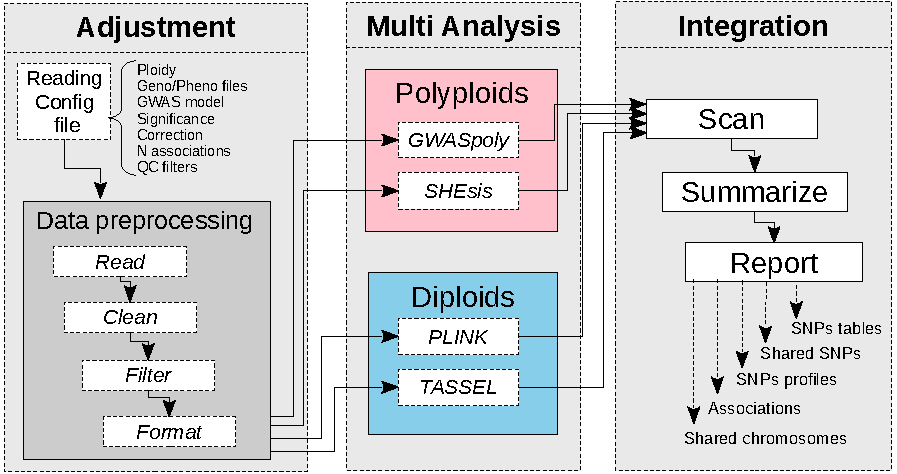
\includegraphics[width=12cm]{images/paper-multiGWAS-flowchart-stages} \caption{\textbf{MultiGWAS flowchart has three steps: adjustment, multi analysis, and integration.} In the first step, the user uploads the input data management, reading the configuration file, and reading and preprocessing the input data (genotype and phenotype). In the second step, the users perform the GWAS analysis, configuring and running the four packages in parallel. And the third step, the user can browse the summarizing and reporting results using different tabular and graphical visualizations.\label{fig:Pipeline}}
\end{figure}

% Preview source code from paragraph 15 to 49


\subsection{Adjustment stage}

MultiGWAS takes as input a configuration file where the user specifies the genomics data along with the parameters that will be used by the four tools. Once the configuration file is read and processed, the genomic data files (genotype and phenotype) are preprocessed by cleaning, filtering, and checking data quality. The output of this stage corresponds to the inputs for the four programs at the Multi Analysis stage.

%genotype/phenotype filenames, genome-wide significance threshold, multiple testing correction methods, GWAS model, number of associations to be reported, and TRUE or FALSE whether to use quality control (QC) filters or not. 

\subsubsection{Reading configuration file\label{section-Reading-configuration-file}}

The configuration file includes the following settings that we briefly describe:% (1) Input genotype and phenotype file names (2) GWAS model, (3) Significance threshold, (4) Correction (5) Quality Control (QC) filters and (6) number of associations to report. 

\paragraph{{Ploidy:}} Numerical value for the ploidy level of the genotype, currently MultiGWAS supports diploids and tetraploids genotypes (2: for diploids, 4: for tetraploids).

\paragraph{{Genotype and phenotype input files:}}

MultiGWAS uses two input files, one for genotype and one for the phenotype. Genotypes files can be either in GWASpoly format (\cite{Rosyara2016}) using SNP markers in rows and samples in columns (Fig. \ref{fig:File-Formats}.a) or Variant Call Format (VCF) (Fig.\ref{fig:File-Formats}.b) which is transformed into GWASpoly format using NGSEP 4.0.2 (\cite{Duitama2019}). The phenotype file contains only one trait and uses a matrix format with the first column for the sample names and the second column for the trait values (Fig. \ref{fig: File-Formats}.c).

\begin{figure}[H]
\begin{centering}
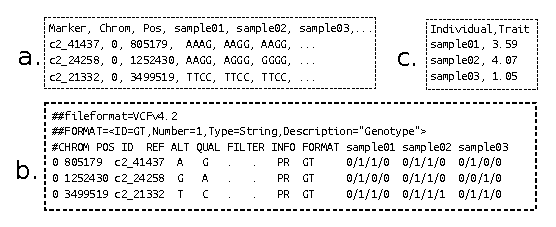
\includegraphics{images/paper-input-files}
\par\end{centering}
\caption{\scriptsize \textbf{{Examples of MultiGWAS input file formats}}. Figures a and b show genotype files in GWASpoly and VCF formats, respectively, while figure c shows a phenotype file in a matrix format. a. Genotype file in GWASpoly format containing column headers and with the first three columns for markers names, chromosomes and positions. The following columns correspond to the marker data of the samples in \textquotedbl{}ACGT\textquotedbl{} format (e.g. AAGG, CCTT for tetraploids, AG, CT for diploids). b. Genotype file in VCF format with metadata (first two lines) and header line. The following lines contain genotype information of the samples for each position. VCF marker data can be encoded as simple genotype calls (GT format field, e.g. 0/0/1/1 for tetraploids or 0/1 for diploids) or using the NGSEP custom format fields (\cite{Duitama2019}): ACN, ADP or BSDP. c. Phenotype file in a matrix format with column headers and sample names followed by their trait values. Both GWASpoly genotype and phenotype files are in CSV (Comma Separated Values) format.).} \label{fig:File-Formats}\protect \\
\end{figure}


\paragraph{GWAS model:}

MultiGWAS is designed to work with quantitative phenotypes and can run GWAS analysis using two types of statistical models that we have called \emph{full} and \emph{naive} models. The \emph{full model} is know in the literature as the Q+K model \cite{Yu2006} and includes control for structure (Q) and relatedness between samples (K), whereas the \emph{naive model} does not include any type of correction. Both models are based on linear regression approaches and variations of them are implemented by the four GWAS packages used by MultiGWAS. The \emph{naive} is modeled with Generalized Linear Models (GLMs, Phenotype + Genotype), and the \emph{full} is modeled with Mixed Linear Models (MLMs, Phenotype + Genotype + Structure + Kinship). The default model used by MultiGWAS is the \emph{full model} (Q+K) \cite{Yu2006}, which is expressed with the following equation:

\[
y=X\beta+S\alpha+Q\nu+Z\mu+e
\]

where $y$ is the vector of observed phenotypes; $\beta$ is a vector of fixed effects other than SNP or population group effects; $\alpha$ is a vector of SNP effects (Quantitative Trait Nucleotides); $\nu$ is a vector of population effects; $\mu$ is a vector of polygene background effects; $e$ is a vector of residual effects; $Q$, modeled as a fixed effect, refers to the incidence matrix for subpopulation covariates relating $y$ to $\nu$; and $X$, $S$ and $Z$ are incidence matrices of 1s and 0s relating $y$ to $\beta$, $\alpha$ and $\mu$, respectively.


\paragraph{Genome-wide significance: }

GWAS searches SNPs associated with the phenotype in a statistically significant manner. A threshold or significance level $\alpha$ is specified and compared with the \emph{p-value} derived for each association score. Standard significance levels are 0.01 or 0.05 \cite{Gumpinger2018,Rosyara2016}, and MultiGWAS uses an $\alpha$ of 0.05 for the four GWAS packages. But the threshold is adjusted according to each package, as some packages as GWASpoly and TASSEL calculates the SNP effect for each genotypic class using different gene action models (see ``Multi analysis stage''). So, the number of tested markers\emph{ }may be different in each model (see below) that results in different \emph{p-value} thresholds.

\paragraph{Multiple testing correction:}

Due to the massive number of statistical tests performed by GWAS, it is necessary to perform a correction method for multiple hypothesis testing and adjusting the \emph{p-value} threshold accordingly. Two common methods for multiple hypothesis testing are the false discovery rate (FDR) and the Bonferroni correction. The latter is the default method used by MultiGWAS, which is one of the most stringent methods. However, instead of adjusting the \emph{p-values,} MultiGWAS adjust the threshold below which a \emph{p-value} is considered significant, that is $\alpha/m$, where $\alpha$ is the significance level and \emph{m }is the number of tested markers from the genotype matrix. 

\paragraph{Number of reported associations: }

Criticism has arisen in considering only statistically significant associations as the only possible correct associations \cite{Thomson2011,Kaler2019}. Many of low \emph{p-value} associations, closer to being significant, are discarded due to the stringent significance levels, and consequently increasing the number of false negatives. To help to analyze both significant and non-significant associations, MultiGWAS provides the option to specify the number of best-ranked associations (lower \emph{p-values}), adding the corresponding \emph{p-value} to each association found. In this way, it is possible to enlarge the number of results, and we can observe replicability in the results for different programs. Nevertheless, we present each association with the corresponding \emph{p-value}.

%  We present the resultant associations in different tables and graphics reported by MultiGWAS (see Figure \ref{fig:-View-Shared-SNPs}). 

\paragraph{Quality control filters:}

A control step is necessary to check the input data for genotype or phenotype errors or poor quality that can lead to spurious GWAS results. MultiGWAS provides the option to select and define thresholds for the following filters that control the data quality: Minor Allele Frequency (MAF), individual missing rate (MIND), SNP missing rate (GENO), and Hardy-Weinberg threshold (HWE):
\begin{itemize}
\item \textbf{MAF of }\textbf{\emph{x:}} filters out SNPs with minor allele frequency below \emph{x} (default 0.01); 
\item \textbf{MIND of }\textbf{\emph{x:}} filters out all individuals with missing genotypes exceeding \emph{x}{*}100\% (default 0.1); 
\item \textbf{GENO of }\textbf{\emph{x:}} filters out SNPs with missing values exceeding \emph{x}{*}100\% (default 0.1); 
\item \textbf{HWE of }\textbf{\emph{x:}} filters out SNPs which have Hardy-Weinberg equilibrium exact test \emph{p-value} below the \emph{x} threshold.
\end{itemize}
MultiGWAS does the MAF filtering, and uses the PLINK package \cite{Gumpinger2018} for the other three filters: MIND, GENO, and HWE.

\paragraph{{GWAS tools:}}
List of names of the four GWAS software to run and integrate into MultiGWAS analysis. They are GWASpoly and SHEsis (designed for polyploid data), and PLINK and TASSEL (designed for diploid data). %\ic{Luis, por favor verifica si GWASpoly y SHEsis son ambos para poliploides o solo tetraploides. Me surgió la duda con SHESIS}.

\subsubsection{Data preprocessing}

Once the configuration file is processed, the genomic data is read and cleaned by selecting individuals present in both genotype and phenotype. Then, individuals and SNPs with poor quality are removed by considering the previous selected quality-control filters and their thresholds, 

At this point, the format \textquotedbl{}ACGT\textquotedbl{} suitable for the polyploid software GWASpoly and SHEsis, is \textquotedbl{}diploidized\textquotedbl{} for PLINK and TASSEL. The homozygous tetraploid genotypes are converted to diploid thus: AAAA\textrightarrow AA, CCCC\textrightarrow CC, GGGG\textrightarrow GG, TTTT\textrightarrow TT. Moreover, for tetraploid heterozygous genotypes, the conversion depends on the reference and alternate alleles calculated for each position (e.g., AAAT \textrightarrow AT, ... ,CCCG\textrightarrow CG). 

After this process, the genomic data, genotype and phenotype, are converted to the specific formats required for each of the four GWAS packages.

\subsection{Multi analysis stage}
MultiGWAS runs in parallel using two types of statistical models specified in the parameters file, the Full model (Q+K) and Naive (i.e., without any control) where Q refers to population structure and K refers to relatedness, calculated by kinship coeficients across individuals (\cite{Sharma2018}). The Full model (Q+K) controls for both population structure and individual relatedness. For population structure, MultiGWAS uses the Principal Component Analysis (PCA) and takes the top five PC as covariates. For relatedness, MultiGWAS uses kinship matrices that TASSEL and GWASpoly calculated separately, and for PLINK and SHEsis, relatedness depends on kinship coefficients calculated with the PLINK 2.0 built-in algorithm (\cite{Chang2015}). 

\subsubsection{GWASpoly\label{subsec_GWASpoly}}
%Editado y revisado por Ivania el 5 de junio
GWASpoly (\cite{Rosyara2016}) is an R package designed for GWAS in polyploid species used in several studies in plants (\cite{Berdugo2017,Ferrao2018,Sharma2018,Yuan2019}). GWASpoly uses a Q+K linear mixed model with biallelic SNPs that account for population structure and relatedness. Also, to calculate the SNP effect for each genotypic class, GWASpoly provides eight gene action models: general, additive, simplex dominant alternative, simplex dominant reference, duplex dominant alternative,duplex dominant, diplo-general, and diplo-additive. As a consequence, the number of statistical test performed can be different in each action model and so thresholds below which the \emph{p-values} are considered significant.

MultiGWAS is using GWASpoly version 1.3 with all gene action models available to find associations. The MultiGWAS reports the top \emph{N} best-ranked (the SNPs with lowest \emph{p-values})  that the user specified in the \emph{N} input configuration file. The \emph{full }model used by GWASpoly includes the population structure and relatedness, which are estimated using the first five principal components and the kinship matrix, respectively, both calculated with the GWASpoly built-in algorithms.

\subsubsection{SHEsis}
%Editado por Ivania el 5 de junio
%Luis por favor revisa que el software SOLO ha sido usado en animales y humanos (que son diploides) y no hay ningún reporte en plantas. En esta afirmación hay que estar muy seguros. Att. Ivania.

SHEsis is a program based on a linear regression model that includes single-locus association analysis, among others. The software design includes polyploid species. However, their use is mainly in diploids animals and humans (\cite{Qiao2015,Meng2019}).

MultiGWAS is using version 1.0, which does not take account for population structure or relatedness. Despite, MultiGWAS externally estimates relatedness for SHEsis by excluding individuals with cryptic first-degree relatedness using the algorithm implemented in PLINK 2.0 (see below).

\subsubsection{PLINK}
%Revisado y editado por Ivania el 5 de junio
PLINK is one of the most extensively used programs for GWAS in humans and any diploid species (\cite{Power2016}). PLINK includes a range of analyses, including univariate GWAS using two-sample tests and linear regression models.

MultiGWAS is using two versions of PLINK: 1.9 and 2.0. Linear regression from PLINK 1.9 performs both naive and full model. For the full model, the software calculates the population structure using the first five principal components calculated with a built-in algorithm integrated into version 1.9. Moreover, version 2.0 calculates the kinship coefficients across individuals using a built-in algorithm that removes the close individuals with first-degree relatedness.

\subsubsection{TASSEL\label{subsec_TASSEL}}
%Revisado y editado por Ivania el 5 de junio
TASSEL is another standard GWAS program based on the Java software developed initially for maize but currently used in several species (\cite{Alvarez2017,Zhang2018}). For the association analysis, TASSEL includes the general linear model (GLM) and mixed linear model (MLM) that accounts for population structure and relatedness. Moreover, as GWASPoly, TASSEL provides three-gene action models to calculate the SNP effect of each genotypic class: general, additive, and dominant, and so the significance threshold depends on each action model.

MultiGWAS is using TASSEL 5.0, with all gene action models used to find the \emph{N} best-ranked associations and reporting the top \emph{N} best-ranked associations (SNPs with lowest \emph{p-values}). Naive GWAS uses the GLM, and full GWAS uses the MLM with two parameters: population structure that uses the first five principal components, and relatedness that uses the kinship matrix with centered IBS method, both calculated with the TASSEL built-in algorithms. 

% Mayo 20 (Por Luis): Pequenhas adiciones y correciones.  

% Sección 2.3 Integration stage: Completada totalmente por Luis G. (Mayo 26)
%Editado por Ivania el 5 de junio
\subsection{Integration stage.}
The outputs resulting from the four GWAS packages are scanned and processed to identify both significant and best-ranked associations with \emph{p-values} lower than and close to a significance threshold, respectively. 

\subsubsection{Calculation of \emph{p-values }and significance thresholds}

GWAS packages compute \emph{p-value }as a measure of association between each SNP and the trait of interest. The real associations are those their \emph{p-value }drops below a predefined significance threshold. However, the four GWAS packages compute differently \emph{p-values} with the consequence to compute them too high or too low. If \emph{p-values} is too high, it would lead to false negatives or SNPs with real associations with the phenotype, but that does not reach the significance threshold. Conversely, if \emph{p-values} are too low, then it would lead to false positives or SNPs with false associations with the phenotype, but that reaches the significance threshold.

To overcome these difficulties, in the case of too high \emph{p-values}, MultiGWAS identifies and reports both significant and best-ranked associations (the ones closest to being statistically significant). Whereas, in the case of too low \emph{p-values}, MultiGWAS provides two methods for adjusting \emph{p-values} and significance threshold: the false discovery rate (FDR) that adjust \emph{p-values, }and the Bonferroni correction, that adjusts the threshold.

By default, MultiGWAS uses the Bonferroni correction that uses the significance level  $\alpha/m$ (defined by the user in the configuration file), and $m$ (the number of tested markers) to adjust the significance threshold in the GWAS study. However, the significance threshold can be different for each GWAS package as some of them use several action models to calculate the SNP effect of each genotypic class. For both PLINK and SHEsis packages, which use only one model, $m$ is equal to the total number of SNPs. However, for both GWASpoly and TASSEL packages, which use eight and three gene action models, respectively, $m$ is equal to the number of tests performed in each model, which is different between models. 

% Jun 11: LuisG: Subsección modificada completamente
% Sección Revisada y editada por Ivania el 18 de junio
% Preview source code from paragraph 71 to 77

\subsubsection{Selection of significant and best-ranked associations}

MultiGWAS reports two groups of associations from the results of the four GWAS packages: the statistically significant associations with \emph{p-values} below a threshold of significance, and the best-ranked associations with the lowest \emph{p-values}, but not reaching the limit to be statistically significant. However, they are representing interesting associations for further analysis (possible false negatives).

In the case of PLINK and SHEsis, which have a unique gene action model, the associations are as described above. But, in the case of GWASpoly and TASSEL, which have eight and three models respectively, MultiGWAS automatically selects the \char`\"{}best gene action model\char`\"{} from each package and takes the associations from it. This selection within GWASPoly and TASSEL has three criteria: the inflation factor (I), the shared SNPs (R) and the significant SNPs (S).

Each gene action model is scored using the following equation: 
\begin{center}
$score(M_{i})=I{}_{i}+R_{i}+S{}_{i}$
\par\end{center}

where $score(M_{i})$ is the score for the gene action model $M_{i}$, with $i$ from $1..k$, for a GWAS package with $k$ gene action models. $I_{i}$ is the score for the inflation factor defined as $I_{i}=1-|1-\lambda(M_{i})|$, where $\lambda(M_{i})$ is the inflation factor for the $M_{i}$ model. $R_{i}$ is the score of the shared SNPs defined as $R_{i}=\sum\limits _{j=1}^{k}{\textstyle |M_{i}\sim M_{j}|}$, where ${\textstyle |M_{i}\sim M_{j}|}$ is the number of SNPs shared between $M_{i}$ and $M_{j}$ models, normalized by the maximum number of SNPs shared between all models. And, $S_{i}$ is the number of significant SNPs of model $M_{i}$ normalized by the total number SNPs shared among all models.

The score is high when an $M_{i}$ model has an inflation factor $\lambda$ close to 1, identifies a high number of shared SNPs, and contains one or more significant SNPs. Conversely, the score is low when the $M_{i}$ model has an inflation factor $\lambda$ either low (close to 0) or high ($\lambda>2$ ), identifies a small number of shared SNPs, and contains 0 or few significant SNPs. In any other case, the score results from the balance among the inflation factor, the number of shared SNPs, and the number of significant SNPs.
%\ic{Luis, revisar si esta última oración quedó con el sentido que querías. Desde "in any other case..."}.



\subsubsection{Integration of results}
%Sección revisada y editada por Ivania el 5 de junio
% Figure several reports
\begin{figure}
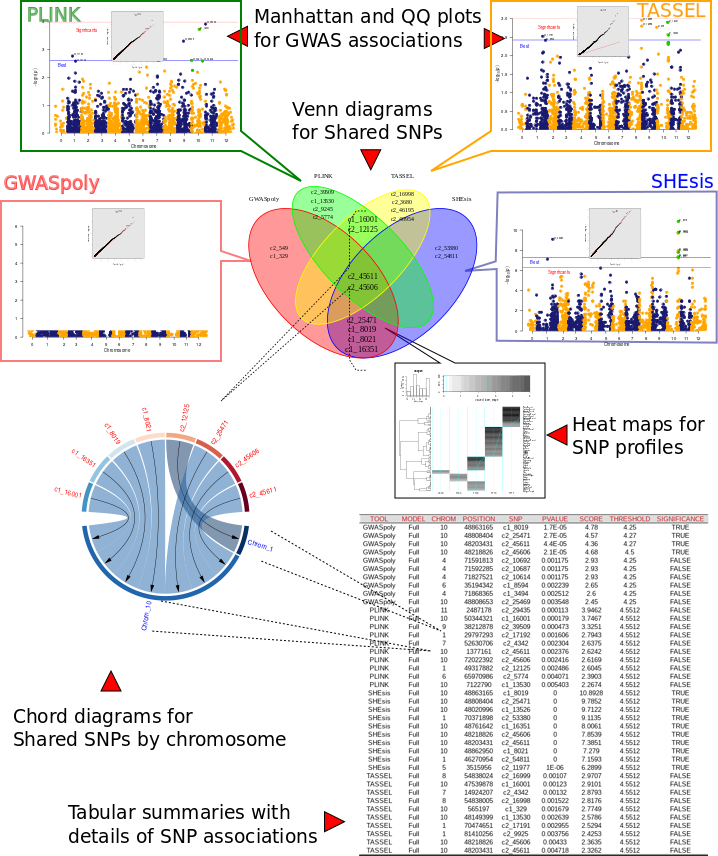
\includegraphics[width=11cm]{images/report-methodologies-all-plots} \caption{\textbf{Reports presented by MultiGWAS}. For each tool, first a QQ plot that assesses the resultant p-values. Second, a Manhattan plot for each tool with two lines, blue and red, respectively, is the lower limit for the best ranked and significative SNPs. We present two Venn diagrams, one for the significative SNPs and one for N best-ranked SNPs of each tool. We show the results for GWAspoly, PLINK, TASSEL, and SHEsis in red, green, yellow, and blue. For each SNP that is in the intersection, thus, that is predicted by more than one tool, we provide an SNP profile. SNPs by chromosome chord diagrams show that the strongest associations are limited to few chromosomes. Furthermore, we present tabular summaries with details of significant and best-ranked associations.\label{fig:Reports} }
\end{figure}
At this stage, MultiGWAS integrates the results to evaluate reproducible results among tools (Fig \ref{fig:Reports}). However, it still reports a summary of the results of each tool: 
\begin{itemize}
\item A Quantile-Quantile (QQ) plots for the resultant \emph{p-values} of each tool and the corresponding inflation factor $\lambda$ to assess the degree of the test statistic inflation. 
\item A Manhattan plot of each tool with two lower thresholds, one for the best-ranked SNPs, and another for the significant SNPs. 
\end{itemize}
To present the replicability, we use two sets: (1) the set of all the significative SNPs provided by each tool and (2) the set of all the best-ranked SNPs. For each set, we present a Venn diagram that shows SNPs predicted exclusively by one tool and intersections that help to identify the SNPs predicted by one, two, three, or all the tools. Also, we provide detailed tables for the two sets.

For each SNP identified more than once, we provide what we call the SNP profile. That is a heat diagram for a specific SNP, where each column is a genotype state AAAA, AAAB, AABB, ABBB, and BBBB. Moreover, each row corresponds to a sample. Samples with close genotypes form together clusters. Thus to generate the clusters, we do not use the phenotype information. However, we present the phenotype information in the figure as the color. This figure visually provides information regarding genotype and phenotype information simultaneously for the whole population. We present colors as tones between white and black for color blind people.

MultiGWAS generates a report, one document with the content previously described. Besides, there is a folder with the individual figures just in case the user needs one.% Preview source code from paragraph 86 to 88

MultiGWAS generates a report, one document with the content previously described. Besides, there is a folder with the individual figures just in case the user needs one (Supplementary Material 1).% \ic{Revisar cómo se pone en la el formato de la revista el supplementary material}.

%PAula: información suplementaria con reporte completo y figuras. Y explicación del reporte

In the following section, we present the results of the functionality of the tool applied on the diversity panel for the tetraploid potato, which has open access for genotyped and phenotyped dataset as part of the USDA-NIFA Solanaceae Coordinated Agricultural Project (SolCAP) (\cite{Hirsch2013}).

% LuisG: Junio 02: Modificado todas las secciones 
%Revisado por Ivania el 19 de junio
\section{Results}
All four GWAS packages adopted by MultiGWAS use linear regression approaches. However, they often produce different association results for the same input. Computed \emph{p-values }for the same set of SNPs are different between packages. Therefore, SNPs with significant \emph{p-values} for one package maybe not significant for the others. Alternatively, well-ranked SNPs in one package may be ranked differently in another. 

To highlight these differences in the results across the four packages, MultiGWAS produces five types of results combining graphics and tables to compare, select, and interpret the set of possible SNPs associated with a trait of interest. The outputs include: 
\begin{itemize}
\item Manhattan and Q-Q plots to show GWAS associations. 
\item Venn diagrams to show associations identified by single or several tools.
\item Heat diagrams to show the genotypic structure of shared SNPs.
\item Chord diagrams to show shared SNPs by chromosomes.
\item Score tables to show detailed information of associations for both summary results from MultiGWAS and particular results from each GWAS
package
\end{itemize}

The complete reports generated by MultiGWAS for both types of analysis, full and naive, applied to the diversity panel of tetraploid potato are in the supplementary information at ~ \url{https://github.com/agrosavia-bioinformatics/multiGWAS-Supplementary}.


% Preview source code from paragraph 103 to 107

\subsection{Manhattan and QQ plots for GWAS associations }

MultiGWAS uses classical Manhattan and Quantile\textendash Quantile plots (QQ plots) to visualize the results of each package. In both plots, the points are the SNPs and their p-values are transformed into scores like $-log_{10}(\mathB{p-values})$ (see Fig. \ref{fig:view-qqmanhattan}). The Manhattan plot shows the strength of association of the SNPs (y-axis) distributed at their genomic location (x-axis), so the higher the score, the stronger the association. At the same time, the QQ plot compares the expected distribution of \emph{p-values} (y-axis) with the observed distribution (x-axis). 

MultiGWAS adds distinctive marks to both plots to identify different types of SNPs: (a) In the Manhattan plots, the significant SNPs are above a red line and the best-ranked SNPs are above a blue line. Also, SNPs shared between packages are coloured green (See Fig. \ref{fig: Table-Shared-SNPs}.b). (b) In the QQ plots, a red diagonal line indicates the expected distribution under the null hypothesis of no association of SNPs with the phenotype, both distributions should coincide, and most SNPs should lie on the diagonal line. Deviations for a large number of SNPs may reflect inflated {\emph{p-values }}due to population structure or cryptic relatedness. But, few SNPs deviate from the diagonal for a truly polygenetic trait (\cite{Power2016}.

\begin{figure}[H]
\begin{centering}
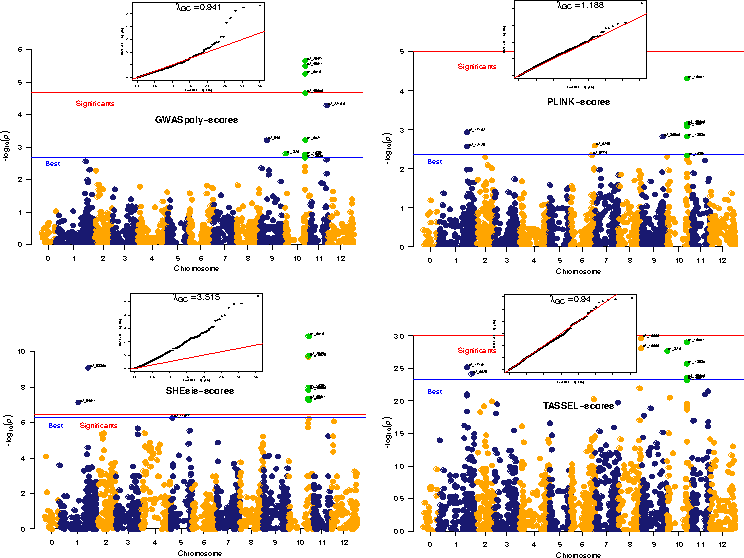
\includegraphics{images/paper-manhattan-QQ-plots}
\par\end{centering}
\caption{\textbf{{Associations in the tetraploid potato dataset.}} MultiGWAS shows the associations identified by the four GWAS packages using Manhattan and QQ plots. The tetraploid potato data showed several SNPs shared between the four software (green dots). The best-ranked SNPs are above the blue line, but only GWASpoly and SHEsis identified significant associations (SNPs above the red line). However, the inflation factor given by SHEsis is too high ($\lambda=3.5$, at the top of the QQ plot), which is observed by the high number of SNPs deviating from the red diagonal of the QQ plot. \label{fig:view-qqmanhattan}}
\end{figure}

\subsection{Tables and Venn diagrams for single and shared SNPs}

MultiGWAS provides tabular and graphic views to report the best-ranked and significant SNPs identified by the four GWAS packages in an integrative way (see Figure \ref{fig:Table-Shared-SNPs}). Both \emph{p-values} and significance levels have been scaled as $-log_{10}(\mathB{p-value})$ to give high scores to the best statistically evaluated SNPs.

First, best-ranked SNPs correspond to the top-scored \emph{N} SNPs, whether they were assessed significant or not by its package, and with\emph{
N} defined by the user in the configuration file. These SNPs appears in both a SNPs table (Figure \ref{fig:Table-Shared-SNPs}.a), and in
a Venn diagram (Figure \ref{fig:Table-Shared-SNPs}.b). The table lists them by package and sorts by decreasing score, whereas the Venn diagram emphasizes if they were best-ranked either in a single package or in several at once (shared). 

Second, the significant SNPs correspond to the ones valued statistically significant by each package. They appear in a Venn diagram (Figure \ref{fig:Table-Shared-SNPs}.c), and in the SNPs table, marked with significance TRUE (T) in the table of the Figure \ref{fig:Table-Shared-SNPs}.a.

\begin{figure}[H]
\begin{centering}
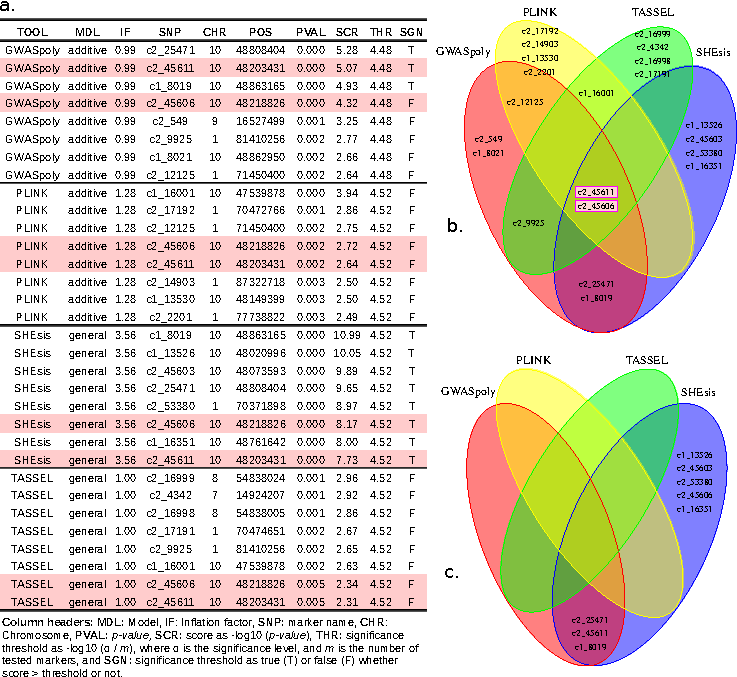
\includegraphics{images/paper-table-venn-best}
\par\end{centering}
\caption{\textbf{Shared SNPs Views. } Tabular and graphical views of SNP associations identified by one or more GWAS packages (shared SNPs). SNPs identified by all packages are marker with red background in all figures. \textbf{(a)} Table with details of the N=9 best-ranked SNPs from each GWAS package. Each row corresponds to a single SNP, and the nine columns are tool name,
the model used by the tool, genomic control factor (inflation factor), SNP name, chromosome, position in the genome, \emph{p-value}, score
as $-log_{10}(\mathB{p-value})$, significance threshold as $-log_{10}(\alpha/m)$ where $\alpha$ is the significance level, and $m$ is the number of
tested markers, and significance as true (T) or false (F) whether score > threshold or not. \textbf{(b)} Venn diagram of the N=9 best-ranked SNPs. SNPs identified by all packages are in the central intersection. Other SNPs identified by more than one packages are in both upper central and lower central intersections. \textbf{(c)} Venn diagram of the significant SNPs (score > threshold). \label{fig:Table-Shared-SNPs}}
\end{figure}

 
%Revisión y edición por Ivania el 26 de junio
\subsection{Heat diagrams for the structure of shared SNPs}

MultiGWAS creates a two-dimensional representation, called the SNP profile, to visualize each trait by individuals and genotypes as rows and columns, respectively (Figure \ref{fig:SNP-profiles}). At the left, the individuals are grouped in a dendrogram by their genotype. At the right, there
is the name or ID of each individual. At the bottom, the genotypes are ordered from left to right, starting from the major to the minor allele (i.e., AAAA, AAAB, AABB, ABBB, BBBB). At the top, there is a description of the trait based on a histogram of frequency (top left) and by an assigned color for each numerical phenotype value using a grayscale (top right). Thus, each individual appears as a
colored line by its phenotype value on its genotype column. For each column, there is a solid cyan line with the mean of each column and a broken cyan line that indicates how far the cell deviates from the
mean.

Because each multiGWAS report shows one specific trait at a time, the histogram and color key will remain the same for all the best-ranked
SNPs.

\begin{figure}[H]
\begin{centering}
\includegraphics{images/paper-heat-maps}
\par\end{centering}
\caption{\textbf{\scriptsize{}SNP profiles. }{\scriptsize{}SNP profiles for
two of the best-ranked significant SNPs shown in the figure \ref{fig:Table-Shared-SNPs}.b.
(a) SNP c2\_45606 best-ranked by the four packages (central intersection
of the Venn diagram Figure \ref{fig:Table-Shared-SNPs}.b) (b) SNP
c1\_8019 best-ranked by the two tetraploid packages (Figure \ref{fig:Table-Shared-SNPs}.b),
and also identified as significant by the same packages (at the bottom
of the Figure \ref{fig:Table-Shared-SNPs}.a). \label{fig:SNP-profiles}}}
\end{figure}

\subsection{Chord diagrams for SNPs by chromosome}
The chord diagrams visualize the location across the genome of the best-ranked associated SNPs shared among the four packages and described in the table \ref{fig: Table-Shared-SNPs}.a.  Thus, in the case of the tetraploid potato, we found that they are located mostly in chromosome 10  (Figure \ref{fig: Chord-diagrams}.a). This visualization complements the manhattan plots from each GWAS package (Figure \ref{fig:Chord-diagrams}.b).


\begin{figure}
\begin{centering}
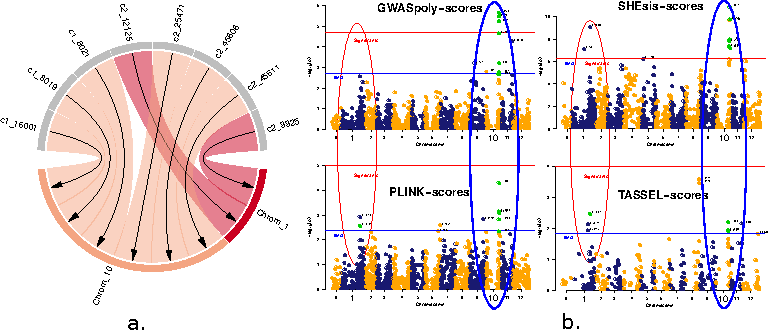
\includegraphics{images/paper-chord-manhattans}
\par\end{centering}
\caption{\textbf{SNPs by chromosome.} The position of best-ranked SNPs across chromosomes using two different visualizations. \textbf{(a)} Chord diagram showing that best-ranked SNPs located in chromosome 10. The SNPs are at the top and the chromosomes at the bottom. The arrows connect the best-ranked SNPs with their position in the chromosomes. \textbf{(b)} Manhattan plots from each GWAS packages showing two important locations of associations, chromosome 1 and chromosome 10, marked with blue and red ellipsis, respectively. \label{fig:Chord-diagrams}}
\end{figure}


% LuisG: Junio 02: Modificado todas las secciones 
%Revisado por Ivania el 26 de junio
\section{Availability and Implementation}

The core of the MultiGWAS tool runs under R and users can interact with the tool by either a command-line interface (CLI) developed in
R or a graphical user interface (GUI) developed in Java (Figure \ref{fig:MultiGWAS-interaction}).
Source code, examples, documentation, and installation instructions are available at \url{https://github.com/agrosavia-bioinformatics/multiGWAS}. 

%Revisado por Ivania el 26 de junio

\subsection{Input parameters}

MutiGWAS uses as the only input a simple configuration text file with the values for the main parameters that drive the analysis. To create the configuration text file, users can choose either a text editor or the MultiGWAS GUI application.  If users prefer a text file, it must have the parameter names and values separated by a colon, filenames enclosed in quotation marks, and TRUE or FALSE values to indicate if filters are applied. If the users prefer the GUI applications, they can create the configuration file using the input parameter view. In any case, this file must have the structure shown in the Figure(Figure \ref{fig:Configuration-file}.a.)

\begin{figure}[H]
\begin{centering}
\includegraphics{images/paper-config-file}
\par\end{centering}
\caption{Configuration file for MultiGWAS. The input parameters include the ploidy level of the organism (2: for diploids, 4: for tetraploids). The input genotype/phenotype filenames. The genome-wide significance threshold. The method for multiple testing correction. The GWAS model. The number of associations to report. The quality control filters choosing TRUE or FALSE. The filters are minor allele frequency, individual missing rate, SNP missing rate, and Hardy-Weinberg threshold. Finally, the GWAS packages selected for the analysis.
\label{fig:Configuration-file}}
\end{figure}

\subsection{Using the command line interface}
The execution of the CLI tool is simple. It only needs to open a Linux console, change to the folder where the configuration file was created, and type the name of the executable tool followed by the the filename of the configuration file, like this:

\begin{lstlisting}[language=bash,basicstyle={\small}]
multiGWAS Test01.config
\end{lstlisting}

Then, the tool starts the execution, showing information on the process in the console window. When it finishes, the results are in a new subfolder called \emph{``out-Test01}.  The results include a complete HTML report containing the different views described in the results section, the source graphics and tables supporting the report, and the preprocessed tables from the results generated by the four GWAS packages used by MultiGWAS.

% Preview source code from paragraph 134 to 137

\subsection{Using the graphical user interface}
The interface allows users to save, load or specify the different input parameters for MultiGWAS in a friendly way (Fig. \ref{fig:MultiGWAS-interaction}. The input parameters correspond to the settings included in the configuration file described in subsection \ref{section-Reading-configuration-file}. It executes by calling the following command from a Linux console:

\begin{lstlisting}[language=bash,basicstyle={\small}]
jmultiGWAS
\end{lstlisting}

\begin{figure}[H]
\begin{centering}
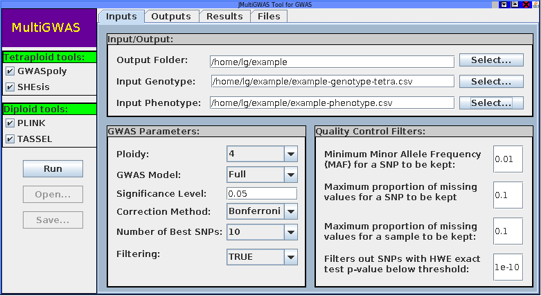
\includegraphics[scale=0.5]{images/paper-implementation-jmultiGWAS}
\par\end{centering}
\caption{\textbf{Main view of the MultiGWAS graphical user interface.}  The interface has a toolbar at the left side and four taps at the top. In the toolbar, users can select the GWAS packages (Two for tetraploids and two for diploids). The analysis starts with the current parameters or loading a previously saved configuration. In the Input tap, users can set the parameters and quality control filters. The Output tap shows the execution of each process. In the Results tap, users can examine an HTML report and browse the source files of each software. Finally, in the Files tap, users can access the produced data across the analysis.}\label{fig:MultiGWAS-interaction} 
\end{figure}

%\ic{Luis, revisa la leyenda de la Fig. 10, si estás conforme con esta descripción de la figura. Traté de hacerla más descriptiva}


\section{Discussion}
%PAULA: Falta discutir un tris los resultados a nivel de informaicón
%PAULA: Tools diploides vs Tools poliploides en poliploides - dosis de los alelos
%IVANIA: Hice una revisión general y me parece que lo escrito por Paula está muy bien, solo corregí algunos detallitos. Sin embargo propongo que la discusión siga el mismo orden que se plantea en la intro sobre los problemas de GWAS en poliploides (replicación, diploidización, integración y modelos de allele dosage). O sino, cambiar la intro con el orden propuesto en la discusión (los datos y la herencia). Como sea, ambas secciones deben coincidir para dar un orden y mostrar específicamente el aporte de MultiGWAS en mejorar esos aspectos (17-Julio).

The reanalysis of potato data with MultiGWAS showed that this tool is handy to improve the GWAS in tetraploid species. Through MultiGWAS performance, we could test its effectiveness to answer some of the challenges associating phenotypic in a polyploid organism. They include the integration and replication among parameters and software, the diploidization of polyploid data, and the incorporation of allele dosage models (\cite{dufresne2014}). 

%PAULA: ventaja de integrar - pvalores inflados de shesis (Balance entre sensitividad y especificidad al integrar)

The main advantage of MultiGWAS is that replicate the GWAS analysis among four software and integrate the results obtained across software, models and parameters. Depending on the software, users usually have to choose between sensitivity or specificity. But using MultiGWAS, users do not have to choose between both approaches because they can observe their effect in the analysis within the same environment.  

Another difficulty for replication among software is the variability of structures for the genomic input data. Currently, the most common format for next-generation sequencing variant data is the VCF (Variant Call Format) (\cite{Danecek2011}; \cite{Ebbert2014}) . One of the advantages of VCF is the versatility to summarize important genome information for hundreds or thousands of individuals and SNP, including information about levels of ploidy. MultiGWAS different from most of GWAS software available allows the VCF as an input (but see VarStats tool in VTC).  

Moreover, the MultiGWAS is the unique tool as far as we know that allows us to compare the effect of diploidized the tetraploid data in the performance of the analysis directly. The graphic outputs are a handy approach to find similar results. The SNP profile allows identifying what the significant associations detected by more than one software are. Furthermore, although MultiGWAS check for significative SNPs based on the p-value, it is essential to go back to the data and check if the SNP is a real association between the genotype and phenotype. For this purpose, the SNP profile gives visual feedback for the accuracy of the association.

%selección del modelo adecuado para cada tool - %Paula: Para polyploides el modo de inheritance es complejo por eso una selección del tool basada en replicabilidad y el factor de inflación es una propuesta justificada

Finally, the MultyGWAS allows comparing among the gene action models that offer GWASPoly and TASSEL.  GWASpoly (\cite{Rosyara2016}) provides models of different types of polyploid gene action including additive, diploidized additive, duplex dominant, simplex dominant, and general. On the other hand, TASSEL (\cite{Bradbury2007}) also models different types of gene action for diploids general, additive and dominant. To choose among models, We propose an automatic selection of the gene action model for both tools based on a balance between three criteria: the inflation factor, the replicability of identified SNPs and the significance of identified SNPs. This inflation index is a new tool for comparison that do not offer either GWASPoly or TASSEL. This automatic strategy will help to understand the gene action model for the trait of interest. Even though the main focus is on the resultant SNPs, the model has assumptions that reflect the gene actions for a specific phenotype.

On the other hand, although MultyGWAS does not solve the uncertainty in the allele dosage and null alleles, However the active comparison among models that MultiGWAS addresses the search of the inheritance mechanisms by comparing among two designed for polysomic inheritance software (\cite{Rosyara2016, Shen2016}) with two software for disomic inheritance (\cite{Purcell2007, Bradbury2007}). Understanding the inheritance mechanisms for polyploids organism is an open question. For autopolyploids, most loci have a polysomic heritage. However, sections of the genome that did not duplicate lead to disomic inheritance for some loci (\cite{ohno1970, lynch2000,dufresne2014}). Thus it is a useful tool for researchers because it looks for significative associations that involve both types of inheritance.



\section{Acknowledgements}
This research was possible thanks to AGROSAVIA five-years macroproject entitled \emph{Investigación en conservación, caracterización y uso de los recursos genéticos vegetales}.
 
We thanks to the Minister of Science, Technology and Innovation of the republic of Colombia (previously COLCIENCIAS), for supporting the postdoctoral researcher L. Garreta at AGROSAVIA during 2019-2020 under the supervision of ICS and PHRH, (Grant number 811-2019). The editorial of AGROSAVIA gave for finatial supporting for this publication. Finally to Andres J. Cortes for his valuable comments to improve this manuscript.
% for supporting the postdoctoral researcher L.Garreta at AGROSAVIA during 2019-2020 under the supervision of ICS and PHRH. 

%\bibliographystyle{apalike}
%\bibliography{multiGWAS}

%\printbibliography
%\bibliographystyle{unsrt}
%\bibliography{mutiGWAS}

\end{document}
